\chapter{Skupinové adresy}
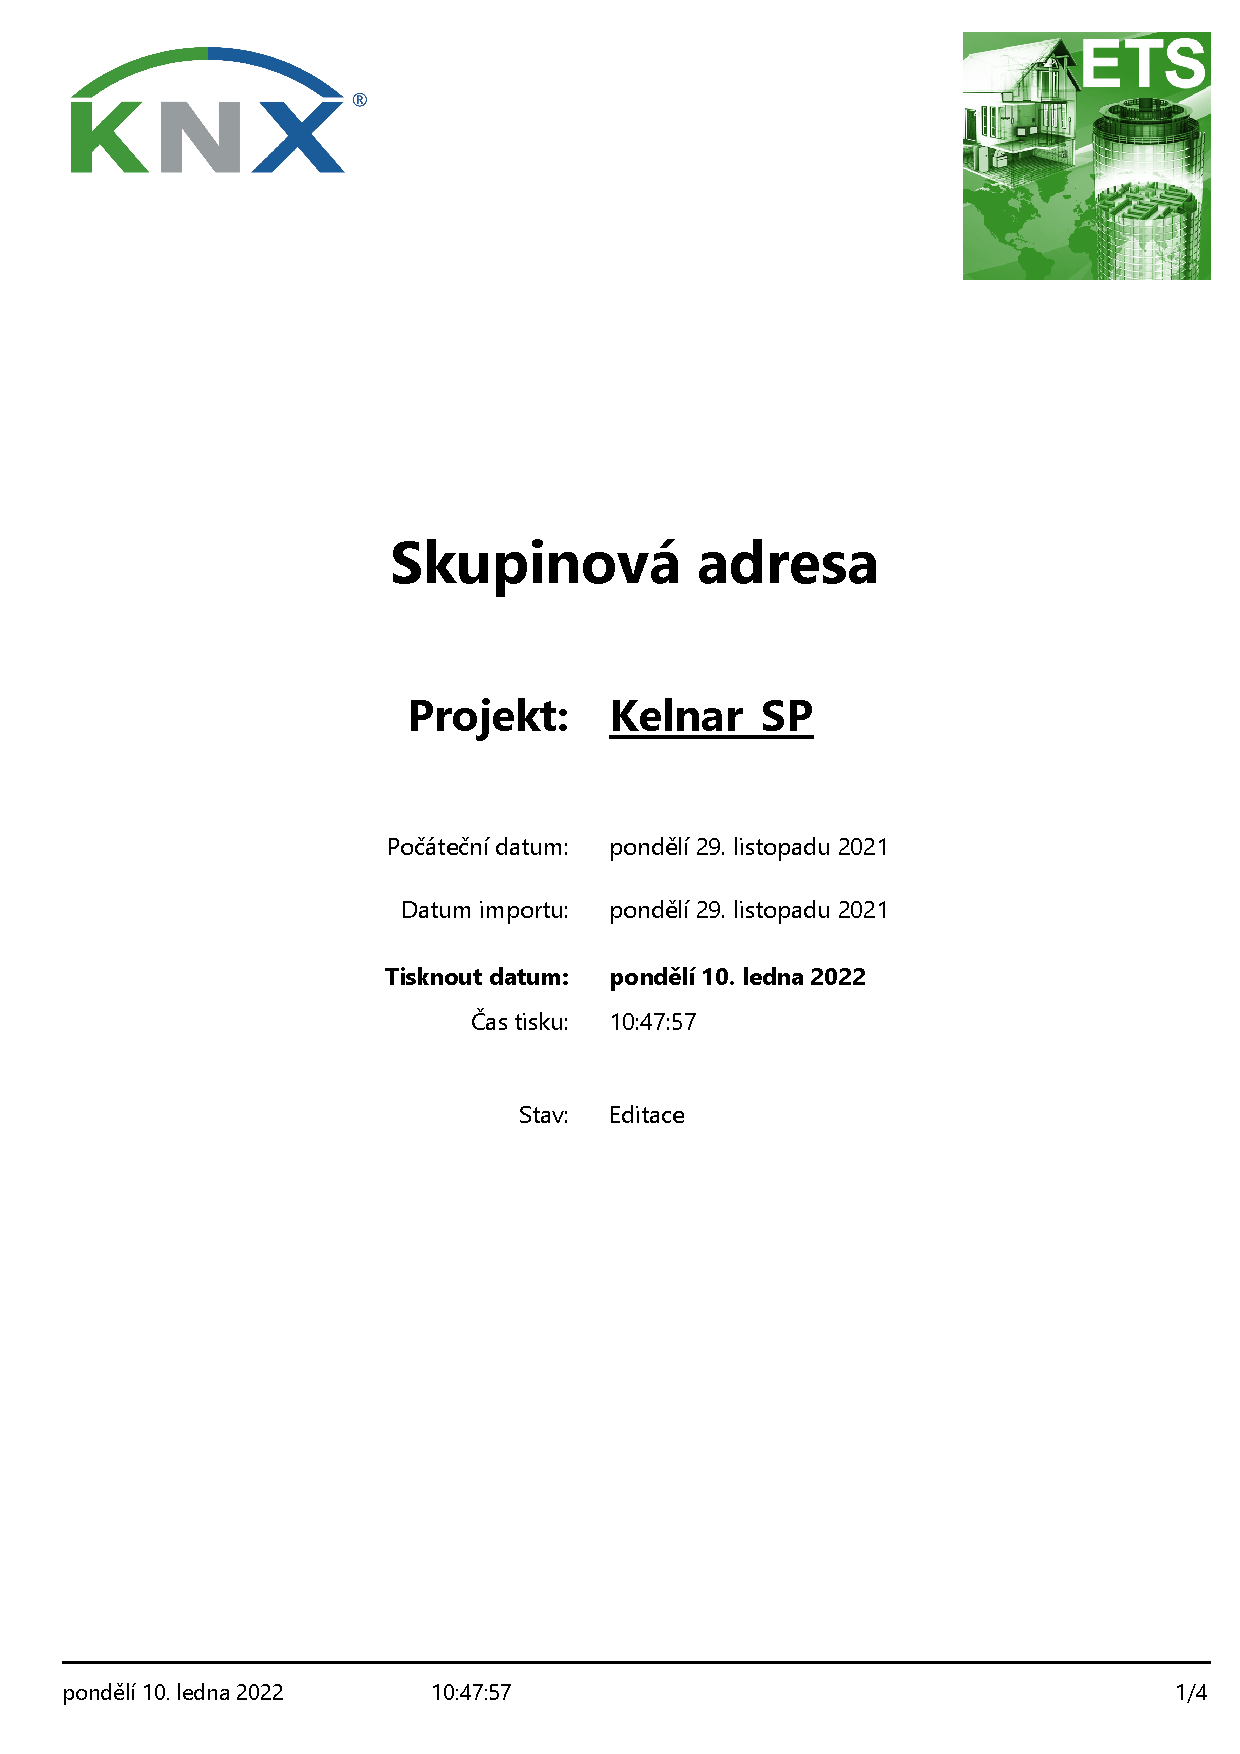
\includepdf[pages = 1]{pdf/GroupAddressesReport}
\includepdf[pages = 2]{pdf/GroupAddressesReport}
\includepdf[pages = 3]{pdf/GroupAddressesReport}
\includepdf[pages = 4]{pdf/GroupAddressesReport}
\chapter{Definice funkčního bloku fbRoomTempMod}
\begin{lstlisting}[language=ST]
FUNCTION_BLOCK fbRoomTempMod
(*Simulace změny teploty v pokojích
*)
  VAR_INPUT
    Heat_1       : BOOl; // Topení vstup 1 [-]
    Heat_1_WATTS : REAL; // Topení výkon 1 [W] => [J/s]
    Heat_2       : BOOL; // Topení vstup 2 [-]
    Heat_2_WATTS : REAL; // Topení výkon 2 [W] => [J/s]
    Cold_1       : BOOl; // Klimatizace vstup 1 [-]
    Cold_1_WATTS : REAL; // Klimatizace výkon 1 [W] => [J/s]
    Cold_2       : BOOL; // Klimatizace vstup 2 [-]
    Cold_2_WATTS : REAL; // Klimatizace výkon 2 [W] => [J/s]
    lenght       : REAL; // délka [m]
    width        : REAL; // šířka [m]
    height       : REAL; // výška [m]
    wall_temp1   : REAL; // Teplota za sousední zdí [deg C]
    wall_temp2   : REAL; // Teplota za sousední zdí [deg C]
    wall_temp3   : REAL; // Teplota za sousední zdí [deg C]
    wall_temp4   : REAL; // Teplota za sousední zdí [deg C]
    floor_temp   : REAL; // Teplota v místnosti pod [deg C]
    ceiling_temp : REAL; // Teplota v místnosti nad [deg C]
    wall_thic1   : REAL; // Šířka zdi1 [m]
    wall_thic2   : REAL; // Šířka zdi2 [m]
    wall_thic3   : REAL; // Šířka zdi3 [m]
    wall_thic4   : REAL; // Šířka zdi4 [m]
    floor_thic   : REAL; // Šířka podlahy [m]
    ceiling_thic : REAL; // Šířka stropu [m]
    TaskTime     : REAL; // Rychlost tasku [ms]
  END_VAR
  VAR_OUTPUT
    Temperature  : REAL := 20.0; // Teplota na výstupu [deg C]
  END_VAR
  VAR_IN_OUT
  END_VAR
  VAR
    INIT         : BOOL := FALSE; //INIT bloku
    TimeStep     : REAL := 0.0; // Hodnota kroku v ms
    VAir         : REAL := 0.0; // Obsah vzduchu v pokoji [m^3]
    MAir         : REAL := 0.0;  // Váha vzduchu [Kg]
    QAir         : REAL := 0.0; // Energie potřebná ke změně o 1deg C [J]
    RoomTemp     : REAL := 20.0; // Pokojová teplota [deg C]
    DeltaTemp    : REAL := 0.0; // Přírůstek teploty za jeden cyklus [deg C]
    KHeatRise    : REAL := 2.4; // Korekční člen pro rychlosti náběhu topení 1 [-]
    KColdRise    : REAL := 45.0; // Korekční člen pro rychlosti náběhu klimatizace 1 [-]
    KHeatFall1   : REAL := 0.0; // Korekční člen pro rychlost poklesu topení 1 [-]
    KColdFall1   : REAL := 0.0; // Korekční člen pro rychlost poklesu klimatizace 1 [-]
    KHeatFall2   : REAL := 0.0; // Korekční člen pro rychlost poklesu topení 2 [-]
    KColdFall2   : REAL := 0.0; // Korekční člen pro rychlost poklesu klimatizace 2 [-]
    Epsilon      : REAL := 1.0; // Hodnota pod kterou musí být výkon do stanoveného času [-]
    AlphaHeat    : REAL := 0.0; // Výsledek logaritmu pro topení [-]
    AlphaCold    : REAL := 0.0; // Výsledek logaritmu pro klimatizace [-]
    FiTotal      : REAL := 0.0; // Celkový tepelný tok [J/s]
    FiHeat       : REAL := 0.0; // Celkový tepelný tok topení [J/s]
    FiHeatTmp1   : REAL := 0.0; // Tepelný tok topení 1 teď [J/s]
    FiHeatTmp2   : REAL := 0.0; // Tepelný tok topení 2 teď [J/s]
    FiCold       : REAL := 0.0; // Celkový tepelný tok klimatizace [J/s]
    FiColdTmp1   : REAL := 0.0; // Tepelný tok klimatizace 1 teď [J/s]
    FiColdTmp2   : REAL := 0.0; // Tepelný tok klimatizace 2 teď [J/s]
    AreaWall1    : REAL := 0.0; // Plocha zdi 1 [m^2]
    AreaWall2    : REAL := 0.0; // Plocha zdi 2 [m^2]
    AreaWall3    : REAL := 0.0; // Plocha zdi 3 [m^2]
    AreaWall4    : REAL := 0.0; // Plocha zdi 4 [m^2]
    AreaFloor    : REAL := 0.0; // Plocha podlahy [m^2]
    AreaCeiling  : REAL := 0.0; // Plocha stropu [m^2]
  END_VAR
  VAR_TEMP
    DeltaTempWall_1     : REAL := 0; // Rozdíl teplot mezi pokoji 1 [deg C]
    DeltaTempWall_2     : REAL := 0; // Rozdíl teplot mezi pokoji 2 [deg C]
    DeltaTempWall_3     : REAL := 0; // Rozdíl teplot mezi pokoji 3 [deg C]
    DeltaTempWall_4     : REAL := 0; // Rozdíl teplot mezi pokoji 4 [deg C]
    DeltaTempFloor      : REAL := 0; // Rozdíl teplot mezi pokojem a podlahou [deg C]
    DeltaTempCeiling    : REAL := 0; // Rozdíl teplot mezi pokojem a stropem [deg C]
    FiWall_1     : REAL := 0.0; // Tepelný tok mezi pokoji 1 [J/s]
    FiWall_2     : REAL := 0.0; // Tepelný tok mezi pokoji 2 [J/s]
    FiWall_3     : REAL := 0.0; // Tepelný tok mezi pokoji 3 [J/s]
    FiWall_4     : REAL := 0.0; // Tepelný tok mezi pokoji 4 [J/s]
    FiFloor      : REAL := 0.0; // Tepelný tok mezi pokojem a podlahou [J/s]
    FiCeiling    : REAL := 0.0; // Tepelný tok mezi pokojem a stropem [J/s]
  END_VAR
  VAR CONSTANT
    RoAir        : REAL := 1.204; // Hustota vzduchu [Kg/m^3]
    CpAir        : REAL := 1005.0; // Tepelná kapacita vzduchu [J/(kg*K)]
    LambdaBrick  : REAL := 0.4; // Tepelná vodivost cihly [W/(m*K)]
    MaxTemp      : REAL := 24.0; // Maximální teplota [deg C]
    MinTemp      : REAL := 16.0; // Minimální teplota [deg C]
    TimeRise     : REAL := 15.0; // Čas náběhu výkonu [s]
    TimeFallHeat : REAL := 15.0; // Čas klesání výkonu topení [s]
    TimeFallCold : REAL := 10.0; // Čas klesání výkonu klimatizace [s]
    TargTimeHeat : REAL := 5.06; // Čas na dosažení 80% topení [s]
    TargTimeCold : REAL := 3.29; // Čas na dosažení 80% klimatizace [s]
  END_VAR
IF NOT(INIT) THEN
   TimeStep := TaskTime / 1000.0; // ms => s
END_IF;
(* Výpočet objemu, hmotnosti, energie *)
IF NOT(INIT) THEN
  VAir := lenght * width * height;
  MAir := RoAir * VAir;
  QAir := MAir * CpAir;
END_IF;

(* Výpočet ploch *)
IF NOT(INIT) THEN
  AreaWall1 := height * width;
  AreaWall2 := height * width;
  AreaWall3 := height * lenght;
  AreaWall4 := height * lenght;
  AreaFloor := lenght * width;
  AreaCeiling := lenght * width;
END_IF;

(* Výpočet deltaT *)
DeltaTempWall_1 := wall_temp1 - RoomTemp;
DeltaTempWall_2 := wall_temp2 - RoomTemp;
DeltaTempWall_3 := wall_temp3 - RoomTemp;
DeltaTempWall_4 := wall_temp4 - RoomTemp;
DeltaTempFloor := floor_temp - RoomTemp;
DeltaTempCeiling := ceiling_temp - RoomTemp;

(* Výpočet tepelných toků přes stěny *)
FiWall_1 := (LambdaBrick * AreaWall1 * DeltaTempWall_1) / wall_thic1;
FiWall_2 := (LambdaBrick * AreaWall2 * DeltaTempWall_2) / wall_thic2;
FiWall_3 := (LambdaBrick * AreaWall3 * DeltaTempWall_3) / wall_thic3;
FiWall_4 := (LambdaBrick * AreaWall4 * DeltaTempWall_4) / wall_thic4;
FiFloor := (LambdaBrick * AreaFloor * DeltaTempFloor) / floor_thic;
FiCeiling := (LambdaBrick * AreaCeiling * DeltaTempCeiling) / ceiling_thic;

(* Výpočet korekčních členu *)
IF NOT(INIT) THEN
  KHeatRise := (TimeRise / TargTimeHeat) - 1.0;
  KColdRise := (TimeRise / TargTimeCold) - 1.0;

  KHeatFall1 := (LN(Heat_1_WATTS/Epsilon))/TimeFallHeat;
  KHeatFall2 := (LN(Heat_2_WATTS/Epsilon))/TimeFallHeat;
  KColdFall1 := (LN(Cold_1_WATTS/Epsilon))/TimeFallCold;
  KColdFall2 := (LN(Cold_2_WATTS/Epsilon))/TimeFallCold;
END_IF;

(* Tepelný výkon topení a klimatizace *)
(* Výpočet alfy *)
IF NOT(INIT) THEN
  AlphaHeat := LN(1 + KHeatRise * (TimeStep)) / LN(1 + KHeatRise * TimeRise);
  AlphaCold := LN(1 + KColdRise * (TimeStep)) / LN(1 + KColdRise * TimeRise);
END_IF;

(* Topení 1 *)
IF Heat_1 THEN
  FiHeatTmp1 := FiHeatTmp1 + AlphaHeat * (Heat_1_WATTS - FiHeatTmp1);
ELSE
  FiHeatTmp1 := FiHeatTmp1 * EXP(-KHeatFall1 * (TimeStep));
END_IF;

(* Topení 2 *)
IF Heat_2 THEN
  FiHeatTmp2 := FiHeatTmp2 + AlphaHeat * (Heat_2_WATTS - FiHeatTmp2);
ELSE
  FiHeatTmp2 := FiHeatTmp2 * EXP(-KHeatFall2 * (TimeStep));
END_IF;

(* Klimatizace 1 *)
IF Cold_1 THEN
  FiColdTmp1 := FiColdTmp1 + AlphaCold * (Cold_1_WATTS - FiColdTmp1);
ELSE
  FiColdTmp1 := FiColdTmp1 * EXP(-KColdFall1 * (TimeStep));
END_IF;

(* Klimatizace 2 *)
IF Cold_2 THEN
  FiColdTmp2 := FiColdTmp2 + AlphaCold * (Cold_2_WATTS - FiColdTmp2);
ELSE
  FiColdTmp2 := FiColdTmp2 * EXP(-KColdFall2 * (TimeStep));
END_IF;

(* Suma výkonů *)
FiHeat := FiHeatTmp1 + FiHeatTmp2;
FiCold := FiColdTmp1 + FiColdTmp2;

(* Celkový tepelný tok *)
FiTotal := FiHeat - FiCold + FiWall_1 + FiWall_2 + FiWall_3 + FiWall_4 + FiFloor + FiCeiling;

(* Výpočet přírůstku teploty za task *)
DeltaTemp := (FiTotal / QAir) * TimeStep;
RoomTemp := RoomTemp + DeltaTemp;

(* Výstup *)
Temperature := RoomTemp;

(* NOT INIT *)
INIT := TRUE;
END_FUNCTION_BLOCK
\end{lstlisting}